\chapter{Shannonova kapacita}

Představme si zašuměný komunikační kanál, kterým posíláme zprávy, které jsou složeny ze symbolů (písmen) nějaké konečné abecedy. Vlivem šumu mohou být některé symboly špatně interpretovány a naším cílem je vybrat co největší počet slov délky $k$ tak, aby žádná dvě slova nebyla vlivem šumu zaměnitelná.

Problém si formalizujeme v řeči teorie grafů. Mějme neorientovaný graf $G = (V, E)$, kde množina vrcholů představuje symboly z konečné abecedy a dva vrcholy $x, y$ jsou spojeny hranou, pokud vrchol $x$ může být vlivem šumu zaměněn za $y$.

Maximální počet nezaměnitelných zpráv délky $1$ je roven $\alpha(G)$, kde $\alpha(G)$ značí velikost největší nezávislé množiny v grafu $G$. Pro popis delších zpráv definujeme \textbf{silný součin} $G \cdot H$ grafů $G$ a $H$ následovně:
$$
    V(G \cdot H) = V(G) \times V(H),
$$
\begin{equation*}
    \begin{split}
    E(G \cdot H) = &\left\{ (i,u)(j,v) \mid ij \in E(G) \wedge uv \in E(H) \right\} \cup \\
                   &\left\{ (i,u)(j,v) \mid ij \in E(G) \wedge u = v \right\} \cup \\
                   &\left\{ (i,u)(j,v) \mid i = j \wedge uv \in E(H) \right\}.
    \end{split}
\end{equation*}

\begin{pr}
Pro graf $P_4 = a-b-c-d-e$ je silný součin $P_4 \cdot P_4$ zobrazen na obrázku~\ref{fig:strong_product_P4_P4}. Z obrázku je hezky vidět, že např. zpráva $cd$ (na obrázku červeně) může být zaměněna s $bc$, $bd$, $be$, $cc$, $ce$, $dc$, $dd$ a $de$ (na obrázku oranžově). Podobně pro další zprávy.
\end{pr}

\begin{figure}[h!]
    \centering
    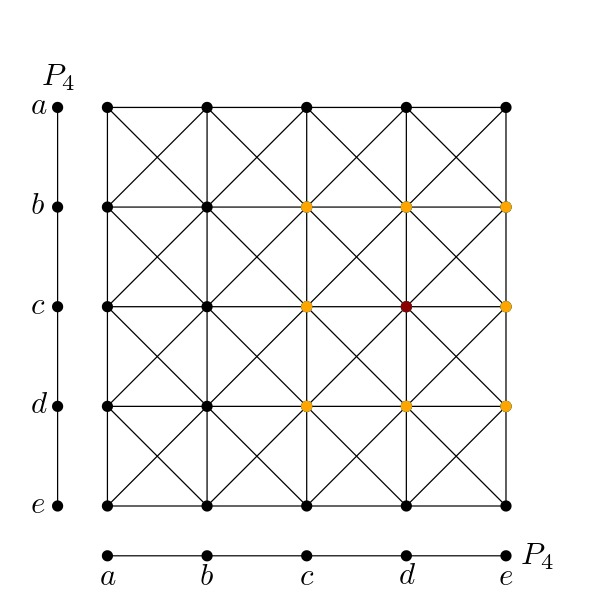
\includegraphics[width=0.5\textwidth]{img/strong_product_P4_P4.png}   
    \caption{$P_4 \cdot P_4$}
    \label{fig:strong_product_P4_P4}
\end{figure}

Pro jednoduchost budeme silný součin $k$ kopií grafu $G$ značit $G^k$. Tedy $\alpha(G^k)$ je maximální počet nezaměnitelných zpráv délky $k$. \textbf{Shannonova kapacita} grafu $G$ je číslo
$$
    \Theta(G) = \lim_{k \rightarrow +\infty} \alpha(G^k)^{1/k}.
$$